\subsubsection*{3.20}
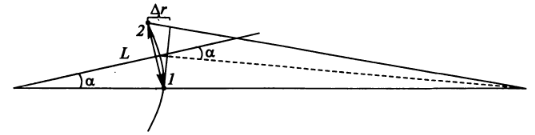
\includegraphics{parts/img/3_20.png}
На рисунке показано положение антенн (1 и 2) при повороте Земли на угол $\alpha$. Разность хода сигнала до антенн при малом угле $\alpha$ равна $\Delta r = L \sin \alpha$. Так как напряжение на контуре пропорционально квадратному корню из интенсивности, то т.к. $I = 2I_0\left[ 1 + \cos (k \Delta r)\right] $, то
\begin{equation*}
	U= U_0 \left[ \cos (k \Delta r/2)\right]  = U_0\left[ \cos(\pi L \sin \alpha / \lambda)\right]  = U_0 \cos \omega t
\end{equation*}
При малых $\alpha$ имеем $\sin \alpha \approx \alpha = \omega_з t$. Таким образом период изменения амплитуды напряжения
\begin{equation*}
	T = 2\pi / \omega = \lambda T_з / (\pi L) = 2,3 мин
\end{equation*}